\documentclass[10pt,a4paper]{article}
\usepackage[T1]{fontenc}
\usepackage[brazil]{babel}
\usepackage[utf8]{inputenc}


\usepackage{ae,aecompl}
\usepackage{pslatex}
\usepackage{epsfig}
\usepackage{geometry}
\usepackage{url}
\usepackage{textcomp}
\usepackage{ae}
\usepackage{subfig}
\usepackage{indentfirst}
\usepackage{textcomp}
\usepackage{color}
\usepackage{setspace}
\usepackage{verbatim}
\usepackage{amsmath}
\usepackage{enumitem}


\include{abaco} 

\renewcommand{\labelenumi}{\arabic{enumi}.}
\renewcommand{\labelenumii}{\arabic{enumi}. \arabic{enumii}}

\onehalfspacing
\begin{document}

% CAPA
\thispagestyle{empty}

\begin{minipage}[h]{0.10\linewidth}
  \ABACO{1}{9}{6}{9}{0.5} 
\end{minipage}
\begin{minipage}[h!]{0.7\linewidth}
  \vspace*{\fill}
  \centering
  {\large \textbf{UNIVERSIDADE~ESTADUAL~DE~CAMPINAS}}\\ 
  {\large INSTITUTO~DE~COMPUTAÇÃO}                   
  \vspace*{\fill} 
\end{minipage}
\\\vspace{0.5cm}

\begin{center} 
  \rule{11.0cm}{0.4pt}\vspace*{-\baselineskip}\vspace{-2.0pt}
  \rule{11.0cm}{1.6pt} \\
  {\large \textsc{Geração de imagens interna do tronco de árvores}}\vspace{-7pt}
  \rule{11.0cm}{0.4pt}\vspace*{-\baselineskip}\vspace{3.2pt} \rule{11.0cm}{1.6pt}\\
  {\textsl{Terceiro projeto de MC920 }}
  \\\vspace{1cm}
  \begin{tabular}{ll}
    Lucas Katayama & \textbf{RA}: 071574\\
    Zhenlei Ji     & \textbf{RA}: 74433\\
    Tiago Chedraoui Silva        & \textbf{RA}: 082941\\
  \end{tabular}
\end{center}
\vspace{0.5cm}
\begin{abstract}

  Métodos acústicos são muito utilizados na detecção de defeitos internos nos mais diferentes
  materiais sendo um deles a madeira. No caso do ultrassom, a propagação
  de ondas é afetada pela presença de materiais com diferentes características de impedância
  acústica ou pela presença de vazios, fazendo com que a velocidade de propagação da onda
  sofra variações. Essas variações podem ser utilizadas em correlações com propriedades ou
  condição interna do material. 

  O objetivo desse trabalho é a avaliar a geração de imagens representativas da condição interna do tronco de árvores através de dados fornecidos pelo uso do ultrassom como ferramenta para a detecção de árvores com presença de ocos.\end{abstract}

\tableofcontents
\newpage 
% \doublespacing

\section{Introdução e Motivação}
Uma das razões para o baixo rendimento de uma árvore é a presença de ocos.
Algumas espécies de valor comercial ou estratégico possuem ocos, o que
inviabiliza economicamente a extração de madeira para o setor madeireiro,
trazendo prejuízos aos produtores que exploram de forma legal a floresta\cite{Proj}.

Atualmente, a detecção da existência de ocos na madeira é realilzada através da utilização de ultrassom um tipo métodos acústicos de propagação de ondas que é afetada pela presença de vazios uma vez que a onda tende a percorrer o meio material.  
Devido ao oco na madeira, a velocidade de propagação da onda
sofre variações que podem ser utilizadas para a reconstrução da imagem de uma tora.

A partir das velocidades fornecidas pelo ultrassom Uslab com transdutores piezoelétricos de faces planas e de frequências de 45kHz, que foi aplicadas sobre amostras de troncos de Pequiá (Aspidosperma desmanthum) cujos ocos possuiam diversos tamanhos de raio, criou-se uma reconstrução das imagens das toras.

\section{Métodos}

Desenvolveu-se na linguagem Matlab\cite{MAT} um programa que dados as
coordenadas e velocidade do ultrassom era possível criar uma imagem
representativa dos buracos e seus respectivos tamanhos.

\subsection{As projeções}

Para a reconstrução da imagem foi fornecidas duas tabelas de dados que
apresentam os dados obtidos através da utilização do ultrassom.

A primeira tabela refere-se a uma malha reticulada,  cuja leitura foi
realizada na na horizontal e vertical (figura \ref{fig:malha1}).
Já a segunda tabela refere-se a uma malha de difração (figura \ref{fig:malha2}).

\begin{figure}[h!]
  \begin{center}
    \leavevmode
    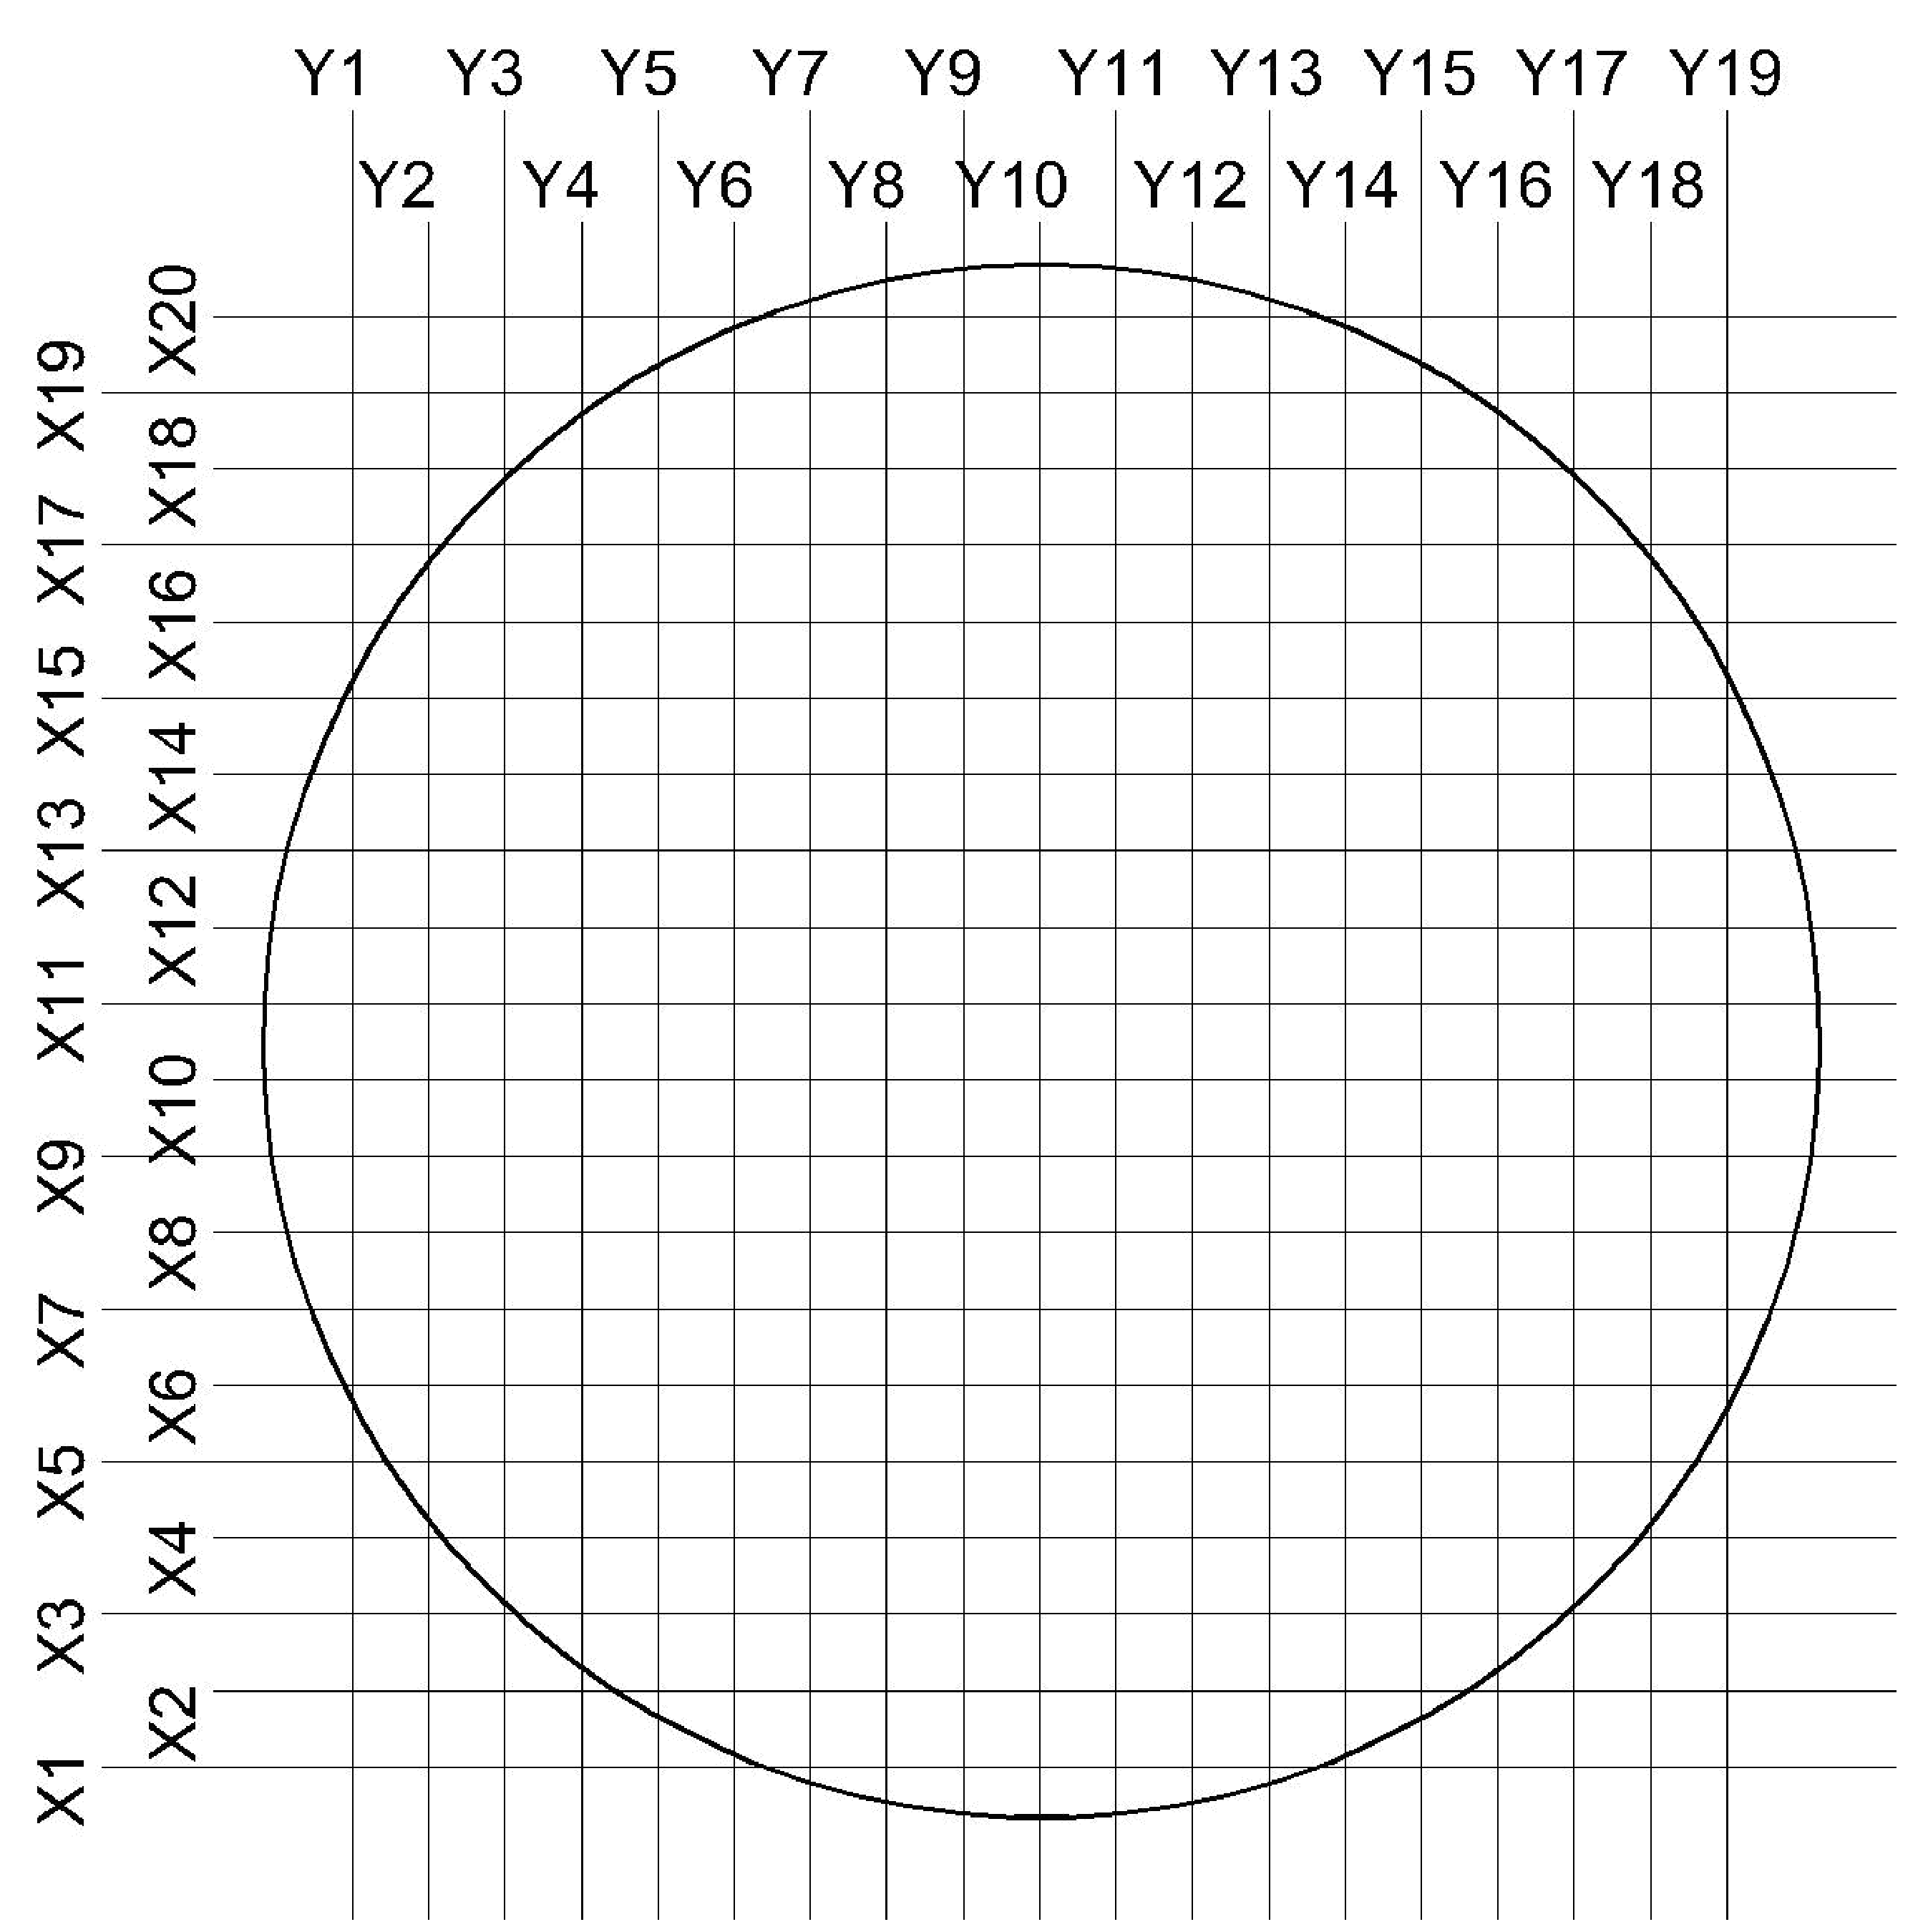
\includegraphics[width=0.3\textwidth]{malha1}
  \end{center}
  \label{fig:malha1}
  \caption{A malha reticulada e as linhas de medição na horizontal e vertical.}
\end{figure}

\begin{figure}[h!]
  \begin{center}
    \leavevmode
    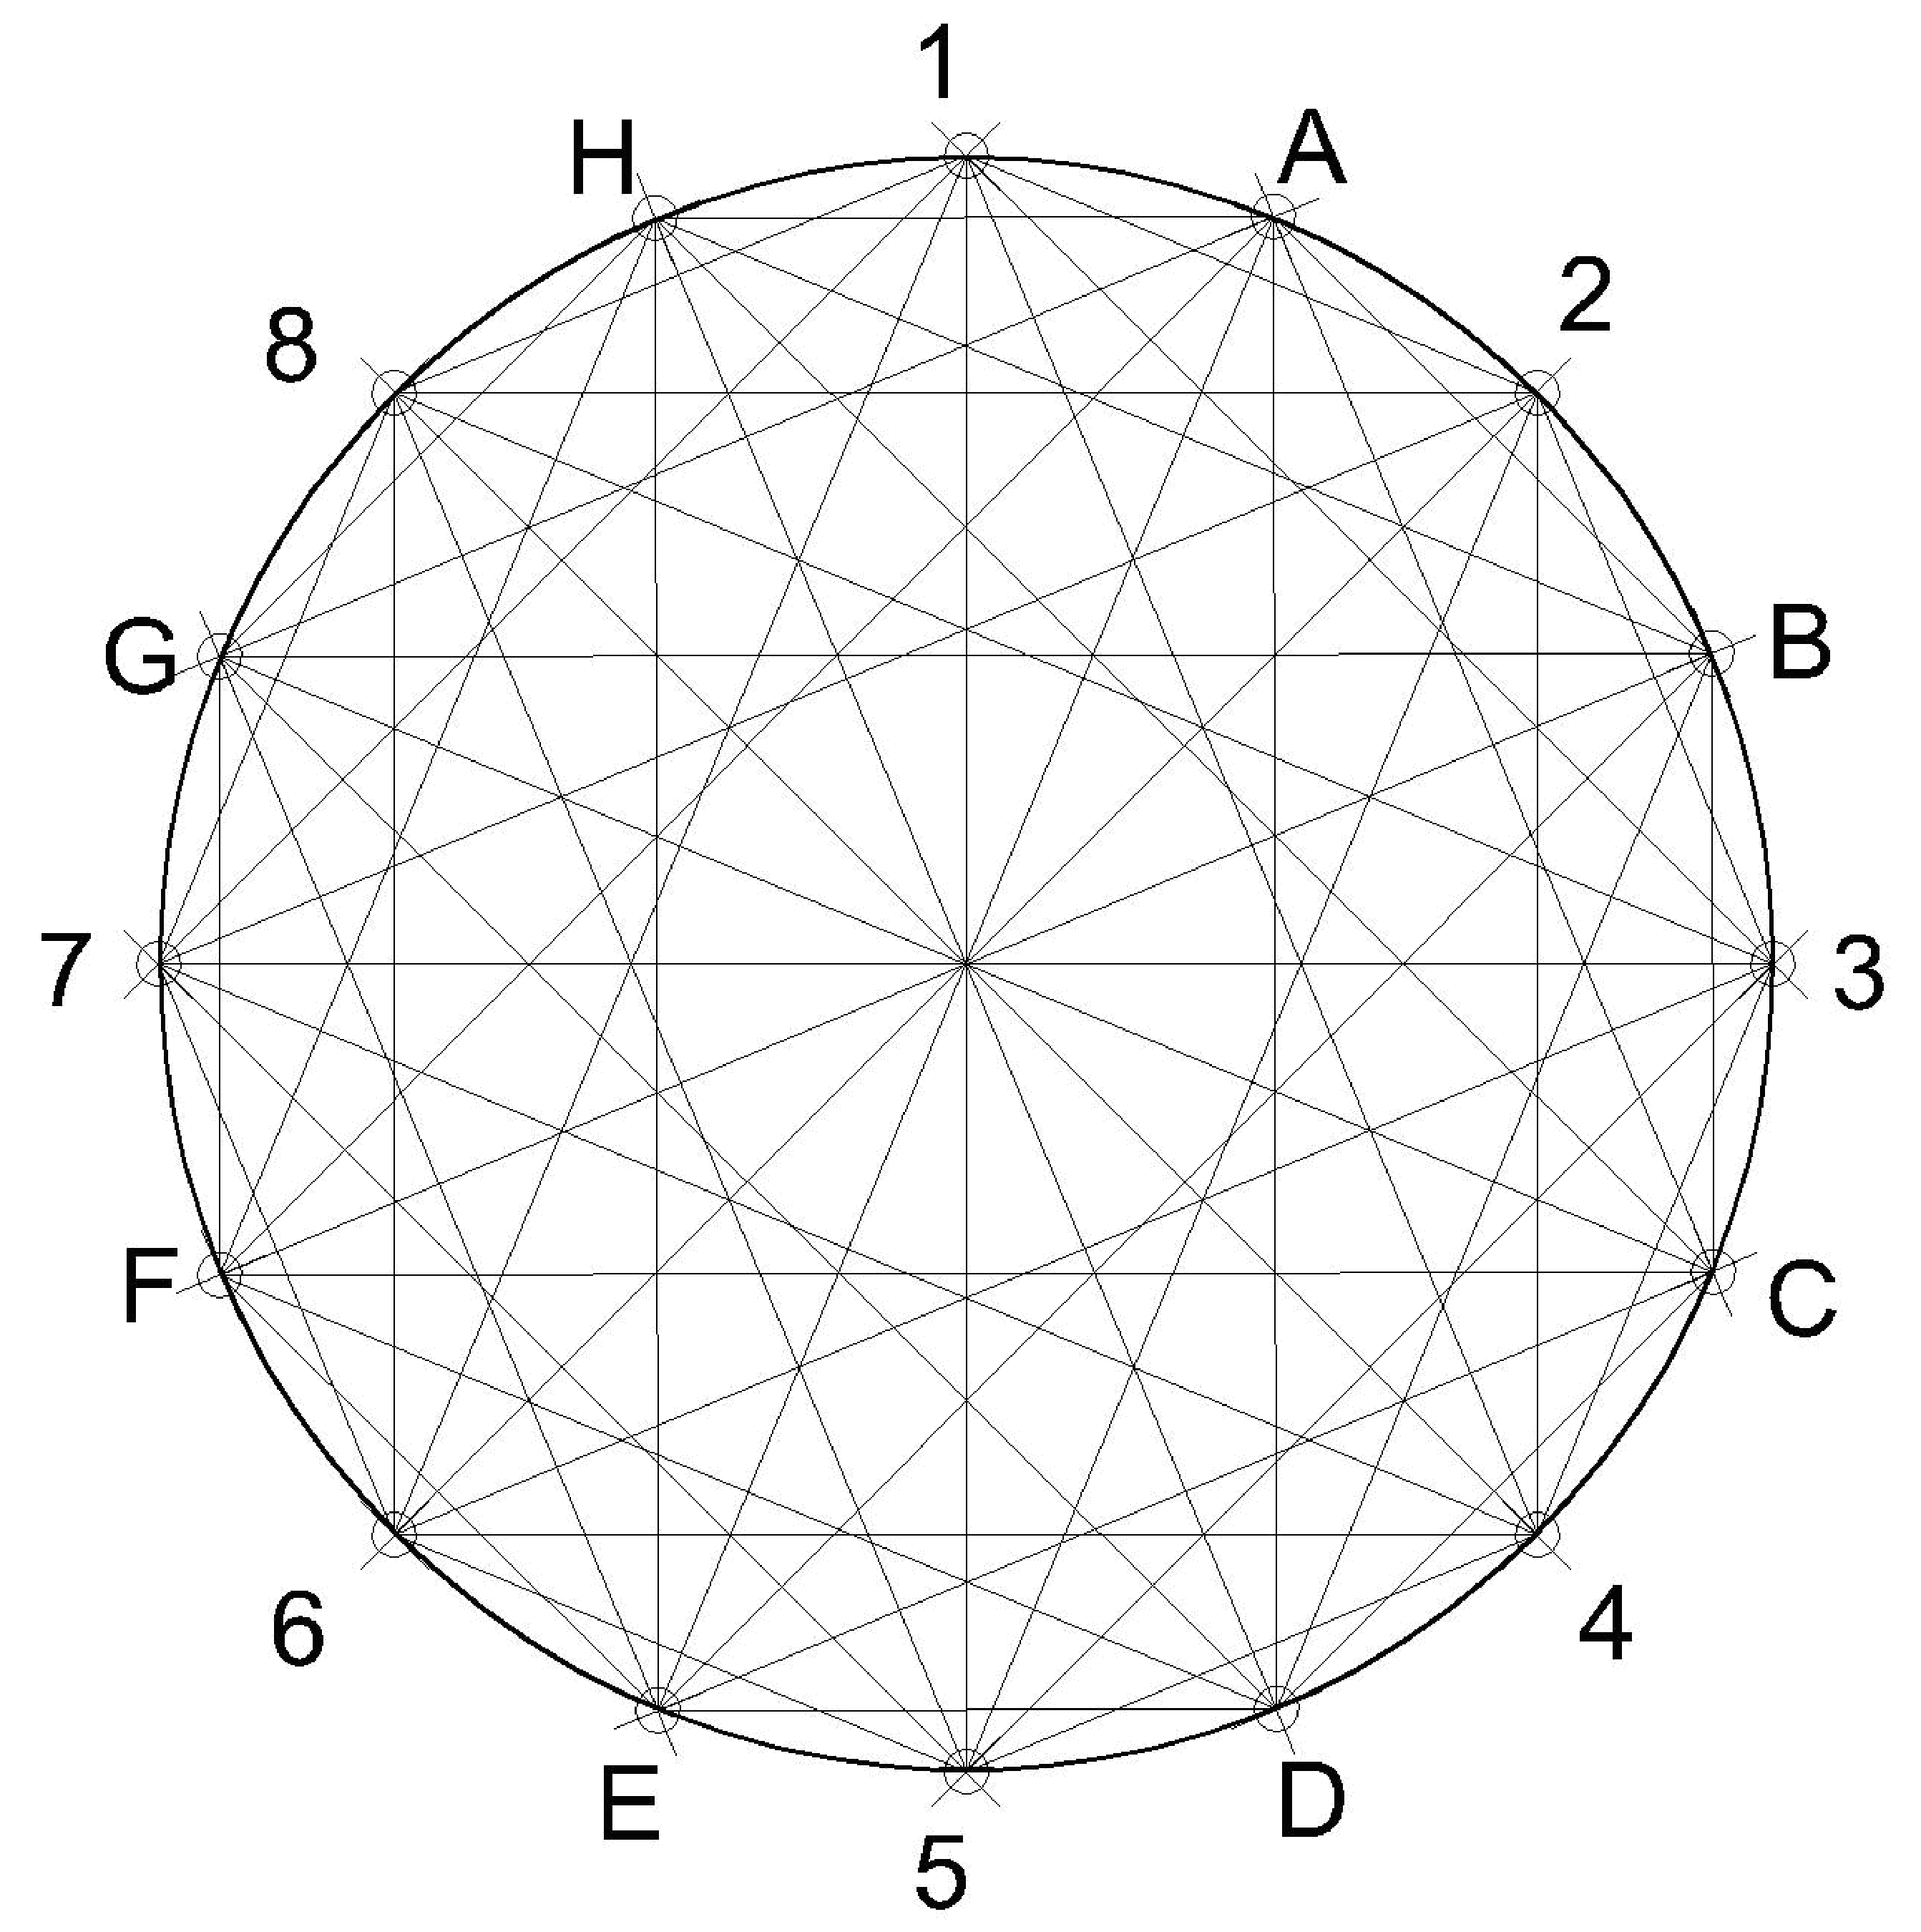
\includegraphics[width=0.3\textwidth]{malha2}
  \end{center}
  \label{fig:malha2}
  \caption{A malha de difração e as linhas de medição.}
\end{figure}

Infelizmente, os dados fornecidos apresentavam alguns problemas, como
dados que possivelmente estavam errado visto as leis da física.
Por exemplo, para um buraco cada vez maior as velocidades deveriam
diminuir, acontecem em alguns pontos da tabelas justamente o oposto.
Além disso, as coordenadas fornecida para as malhas apresentavam
erros.
O resultado original da malha fornecida pode ser visto abaixo.


\begin{figure}[h!]
  \begin{center}
    \leavevmode
    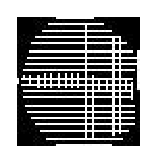
\includegraphics[width=0.2\textwidth]{1}
  \end{center}
  \label{fig:malha1}
  \caption{A malha reticulada fornecida nos dados}
\end{figure}

\begin{figure}[h!]
  \begin{center}
    \leavevmode
    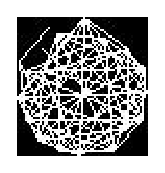
\includegraphics[width=0.2\textwidth]{2}
  \end{center}
  \label{fig:malha2}
  \caption{A malha de difração fornecida nos dados.}
\end{figure}

Para a correção da malhas reticulada tivemos que alterar os pontos de
coordenada do eixo y. O resultado pode ser visto abaixo:


\begin{figure}[h!]
  \begin{center}
    \leavevmode
    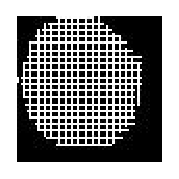
\includegraphics[width=0.2\textwidth]{1novo}
  \end{center}
  \label{fig:malha2}
  \caption{A malha reticulada corrigida.}
\end{figure}

\section{Resultados}

\subsection{Malha reticulada}
\begin{figure}[h!]
\subfloat[0\%]{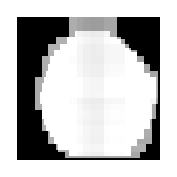
\includegraphics[width=0.1\textwidth]{bv0}}
\hspace{5mm}
\subfloat[5\%]{
\includegraphics[width=0.1\textwidth]{bv5}}
\hspace{5mm}
\subfloat[10\%]{
\includegraphics[width=0.1\textwidth]{bv10}}
\hspace{5mm}
\subfloat[15\%]{
\includegraphics[width=0.1\textwidth]{bv15}}
\hspace{5mm}
\subfloat[20\%]{
\includegraphics[width=0.1\textwidth]{bv20}}
\hspace{5mm}
\subfloat[25\%]{
\includegraphics[width=0.1\textwidth]{bv25}}
\hspace{5mm}
\subfloat[30\%]{
\includegraphics[width=0.1\textwidth]{bv30}}
\hspace{5mm}
\subfloat[35\%]{\includegraphics[width=0.1\textwidth]{bv35}}
\hspace{5mm}
\subfloat[40\%]{
\includegraphics[width=0.1\textwidth]{bv40}}
\hspace{5mm}
\subfloat[45\%]{
\includegraphics[width=0.1\textwidth]{bv45}}
\hspace{5mm}
\subfloat[50\%]{
\includegraphics[width=0.1\textwidth]{bv50}}
\hspace{5mm}
\subfloat[55\%]{\includegraphics[width=0.1\textwidth]{bv55}}
\hspace{5mm}
\subfloat[60\%]{
\includegraphics[width=0.1\textwidth]{bv60}}
\hspace{5mm}
\subfloat[65\%]{\includegraphics[width=0.1\textwidth]{bv65}}
\hspace{5mm}
\subfloat[70\%]{
\includegraphics[width=0.1\textwidth]{bv70}}
\hspace{5mm}
\subfloat[75\%]{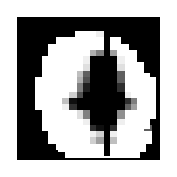
\includegraphics[width=0.1\textwidth]{bv75}}
\hspace{5mm}
\subfloat[80\%]{
\includegraphics[width=0.1\textwidth]{bv80}}
\hspace{5mm}
\subfloat[85\%]{\includegraphics[width=0.1\textwidth]{bv85}}
\hspace{5mm}
\subfloat[90\%]{
\includegraphics[width=0.1\textwidth]{bv90}}

\caption{Resultado malha reticulada}
\end{figure}


\subsection{Malha de difração}

\begin{figure}[h!]
\subfloat[90\%]{\includegraphics[width=0.1\textwidth]{imagem1}}
\hspace{5mm}
\subfloat[85\%]{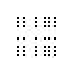
\includegraphics[width=0.1\textwidth]{imagem2}}
\hspace{5mm}
\subfloat[80\%]{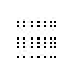
\includegraphics[width=0.1\textwidth]{imagem3}}
\hspace{5mm}
\subfloat[75\%]{\includegraphics[width=0.1\textwidth]{imagem4}}
\hspace{5mm}
\subfloat[70\%]{\includegraphics[width=0.1\textwidth]{imagem5}}
\hspace{5mm}
\subfloat[65\%]{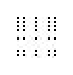
\includegraphics[width=0.1\textwidth]{imagem6}}
\hspace{5mm}
\subfloat[60\%]{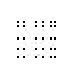
\includegraphics[width=0.1\textwidth]{imagem7}}
\hspace{5mm}
\subfloat[55\%]{\includegraphics[width=0.1\textwidth]{imagem8}}
\hspace{5mm}
\subfloat[50\%]{\includegraphics[width=0.1\textwidth]{imagem9}}
\hspace{5mm}
\subfloat[45\%]{\includegraphics[width=0.1\textwidth]{imagem10}}
\hspace{5mm}
\subfloat[40\%]{\includegraphics[width=0.1\textwidth]{imagem11}}
\hspace{5mm}
\subfloat[35\%]{\includegraphics[width=0.1\textwidth]{imagem12}}
\hspace{5mm}
\subfloat[30\%]{\includegraphics[width=0.1\textwidth]{imagem13}}
\hspace{5mm}
\subfloat[25\%]{\includegraphics[width=0.1\textwidth]{imagem13}}
\hspace{5mm}
\subfloat[20\%]{\includegraphics[width=0.1\textwidth]{imagem14}}
\hspace{5mm}
\subfloat[15\%]{\includegraphics[width=0.1\textwidth]{imagem15}}
\hspace{5mm}
\subfloat[10\%]{\includegraphics[width=0.1\textwidth]{imagem16}}
\hspace{5mm}
\subfloat[5\%]{\includegraphics[width=0.1\textwidth]{imagem17}}
\hspace{5mm}
\subfloat[0\%]{\includegraphics[width=0.1\textwidth]{imagem18}}

\caption{Malha de difração}
\end{figure}

\begin{center}
\begin{figure}[h!]
\begin{center}
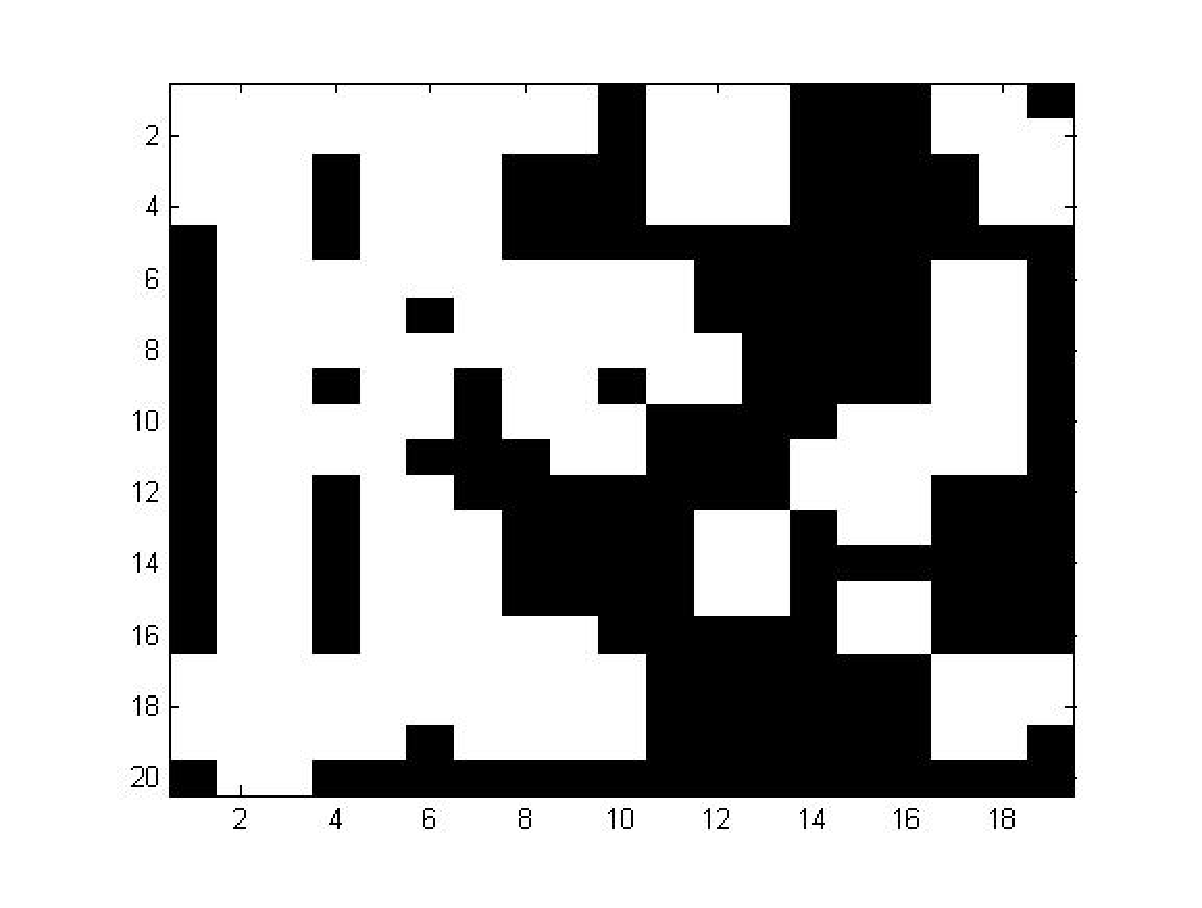
\includegraphics[width=0.2\textwidth]{end}
\caption{Malha de difração - Resultado Final }
\end{center}
\end{figure}
\end{center}

\newpage
\section{Conclusão}

Infelizmente, os dados fornecidos influenciaram consideravelmente nos
resultados. Apesar disso, foi possível rescontruir, para a malha reticulada, possíveis pontos de
buraco, não obtendo, no entando, uma precisão considerável quanto ao seu
diâmatro ou formato. Para que isso fosse possível, mais dados corretos
seriam necessário.
Para o caso de difração tivemos algumas dificuldades, dentre eleas a
idéias de interpolação não surtiu o efeito desejado.


% ******************************************************
% REFERENCIAS BIBLIOGRÁFICAS
% ******************************************************
% \section{Referências}
\bibliographystyle{plain}
\begin{small}
  \bibliography{referencias}
\end{small}

\end{document}
